\chapter*{Практика 6. Модель канала передачи}
\addcontentsline{toc}{chapter}{Практика 6. Модель канала передачи}
\label{ch:6_practice}

\textit{\textbf{Задание:}} Реализовать модель канала с замираниями и АБГШ.

\begin{itemize}
    \item Реализована модель канала со следующими параметрами:
    \begin{itemize}
        \item Несущая частота $f_0 = 1.7$ Гц
        \item Полоса $B = 11$ Гц
        \item Многолучевое распространение ($N_b$ лучей)
        \item Случайные задержки лучей
        \item Добавление АБГШ с заданной мощностью $N_0$
    \end{itemize}
\end{itemize}

\begin{figure}[ht]
    \centering
    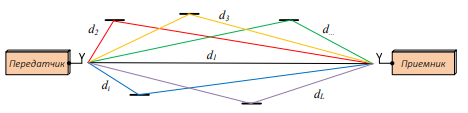
\includegraphics[width=0.8\textwidth]{channel_model.png}
    \caption{Модель канала с замираниями и шумом}
    \label{fig:channel_model}
\end{figure}

\begin{figure}[ht]
    \centering
    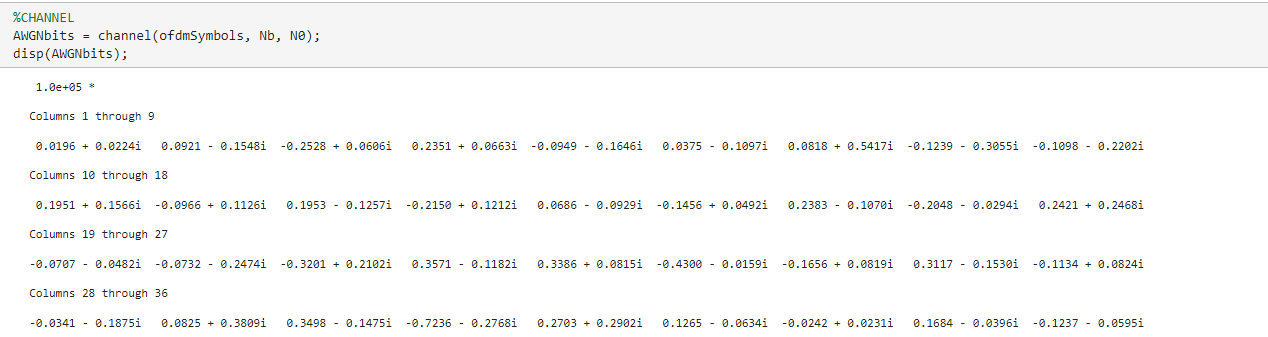
\includegraphics[width=0.8\textwidth]{6practice_result.png}
    \caption{Результат шестой практики}
    \label{fig:6practice_result}
\end{figure}
